\documentclass[a4paper]{article}
\usepackage{amsmath}
\usepackage{amsfonts}
\usepackage{amssymb}
\usepackage{graphicx}
\usepackage{float}

\begin{document}

\noindent \large Auteur: Siebe Haché \\
\noindent \large Studierichting: Informatica \\
\noindent \large Oefeningenreeks 5G nr. 1.5 \\

\medskip
\normalsize

Bereken het volume $V$ dat men bekomt door de functie $f(x) = \dfrac{-1}{x}$ op het interval $[-3, -2]$ om de $x$-as te wentelen.\\

$V = \pi \displaystyle\int_{-3}^{-2} \left( \dfrac{-1}{x} \right)^2 dx$\\

$= \pi \displaystyle\int_{-3}^{-2} \dfrac{1}{x^2} dx$\\

$= \pi \displaystyle\int_{-3}^{-2} x^{-2} dx$\\

$= \pi \left[\dfrac{x^{-1}}{-1}\right]_{-3}^{-2}$\\

$= \pi \left[\dfrac{-1}{x}\right]_{-3}^{-2}$\\

$= \pi \left(\left(\dfrac{-1}{-2}\right) - \left(\dfrac{-1}{-3} \right) \right)$\\

$= \pi \left(\dfrac{1}{2} -\dfrac{1}{3}\right)$\\

$= \pi \left(\dfrac{3}{6} -\dfrac{2}{6}\right)$\\

$= \dfrac{\pi}{6}$\\

\begin{figure}[H]
    \centering
    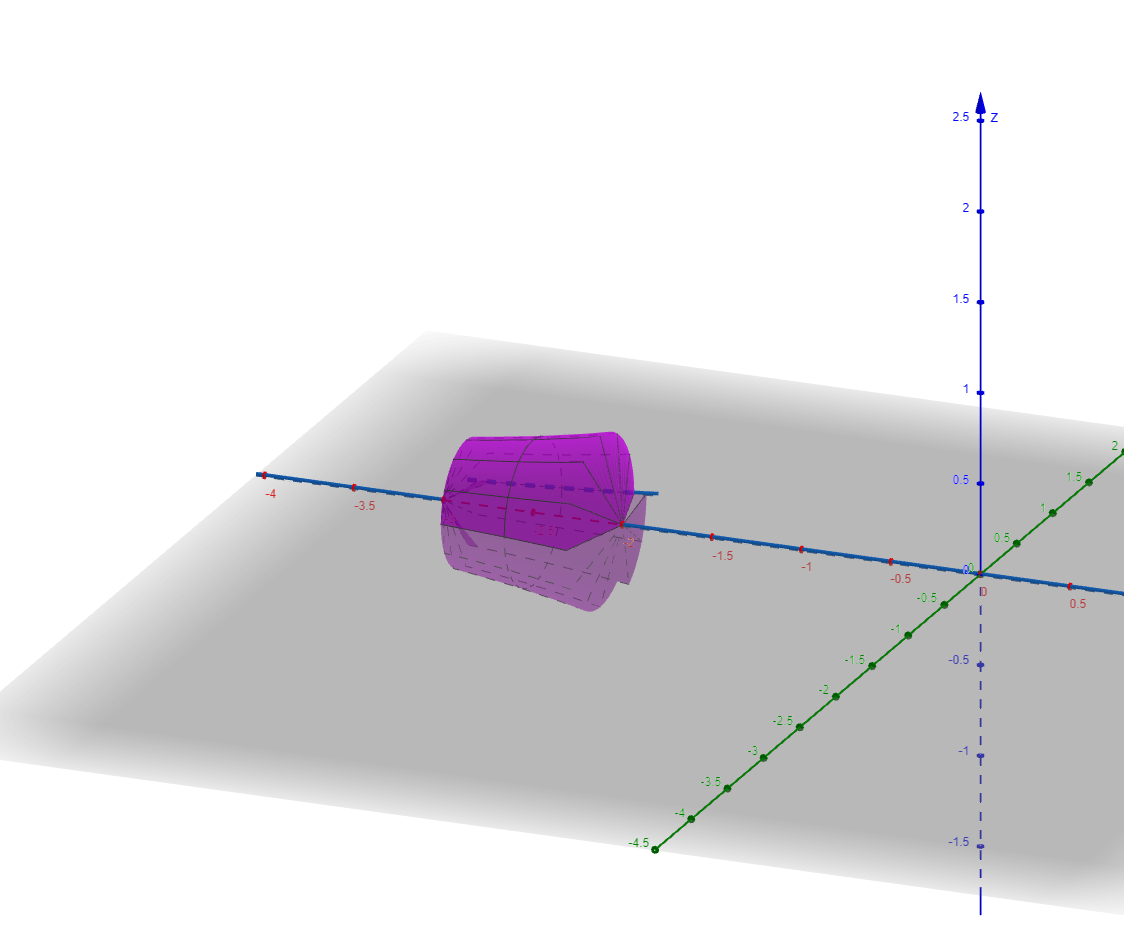
\includegraphics[width=0.6\textwidth]{5G-1.5-siebe.hache.INF.png}
\end{figure}

\begin{thebibliography}{999}
\bibitem{a} Grafiek gemaakt met Desmos
\end{thebibliography}

\end{document}